\section{Experimental Results}

    % Setup dell'esperimento (hardware, software, ecc) con foto
    % Parlare delle tre versioni disponibili (19 gennaio e ultima + differenze) 
    % Bordo nero - divisa in diverse funzioni (crop, enlarge, zoom) (19/01)
    % Bordo nero - unica funzione (26/01)
    % Tolto bordo nero - (ultima versione)
    % Comparison dei risultati in queste versioni (tempo di esecuzione, visione dell'immagine)
    % Discutere le differenze di zooming level in base alla grandezza del ritaglio (in pixel)
    % 
    \subsection{Experimental setup}
    The project has been carried out using a Jetson Nano [\ref{fig:jetson}], a small single-board computer with a quad-core ARM Cortex-A57 CPU and a Maxwell GPU \cite{jetson_nano}. 
    The Jetson Nano is equipped with 4GB of RAM and an SDCard for the Operating System and data storage. The operating system used is Ubuntu 18.04. 

    \begin{figure}[h]
        \centering
        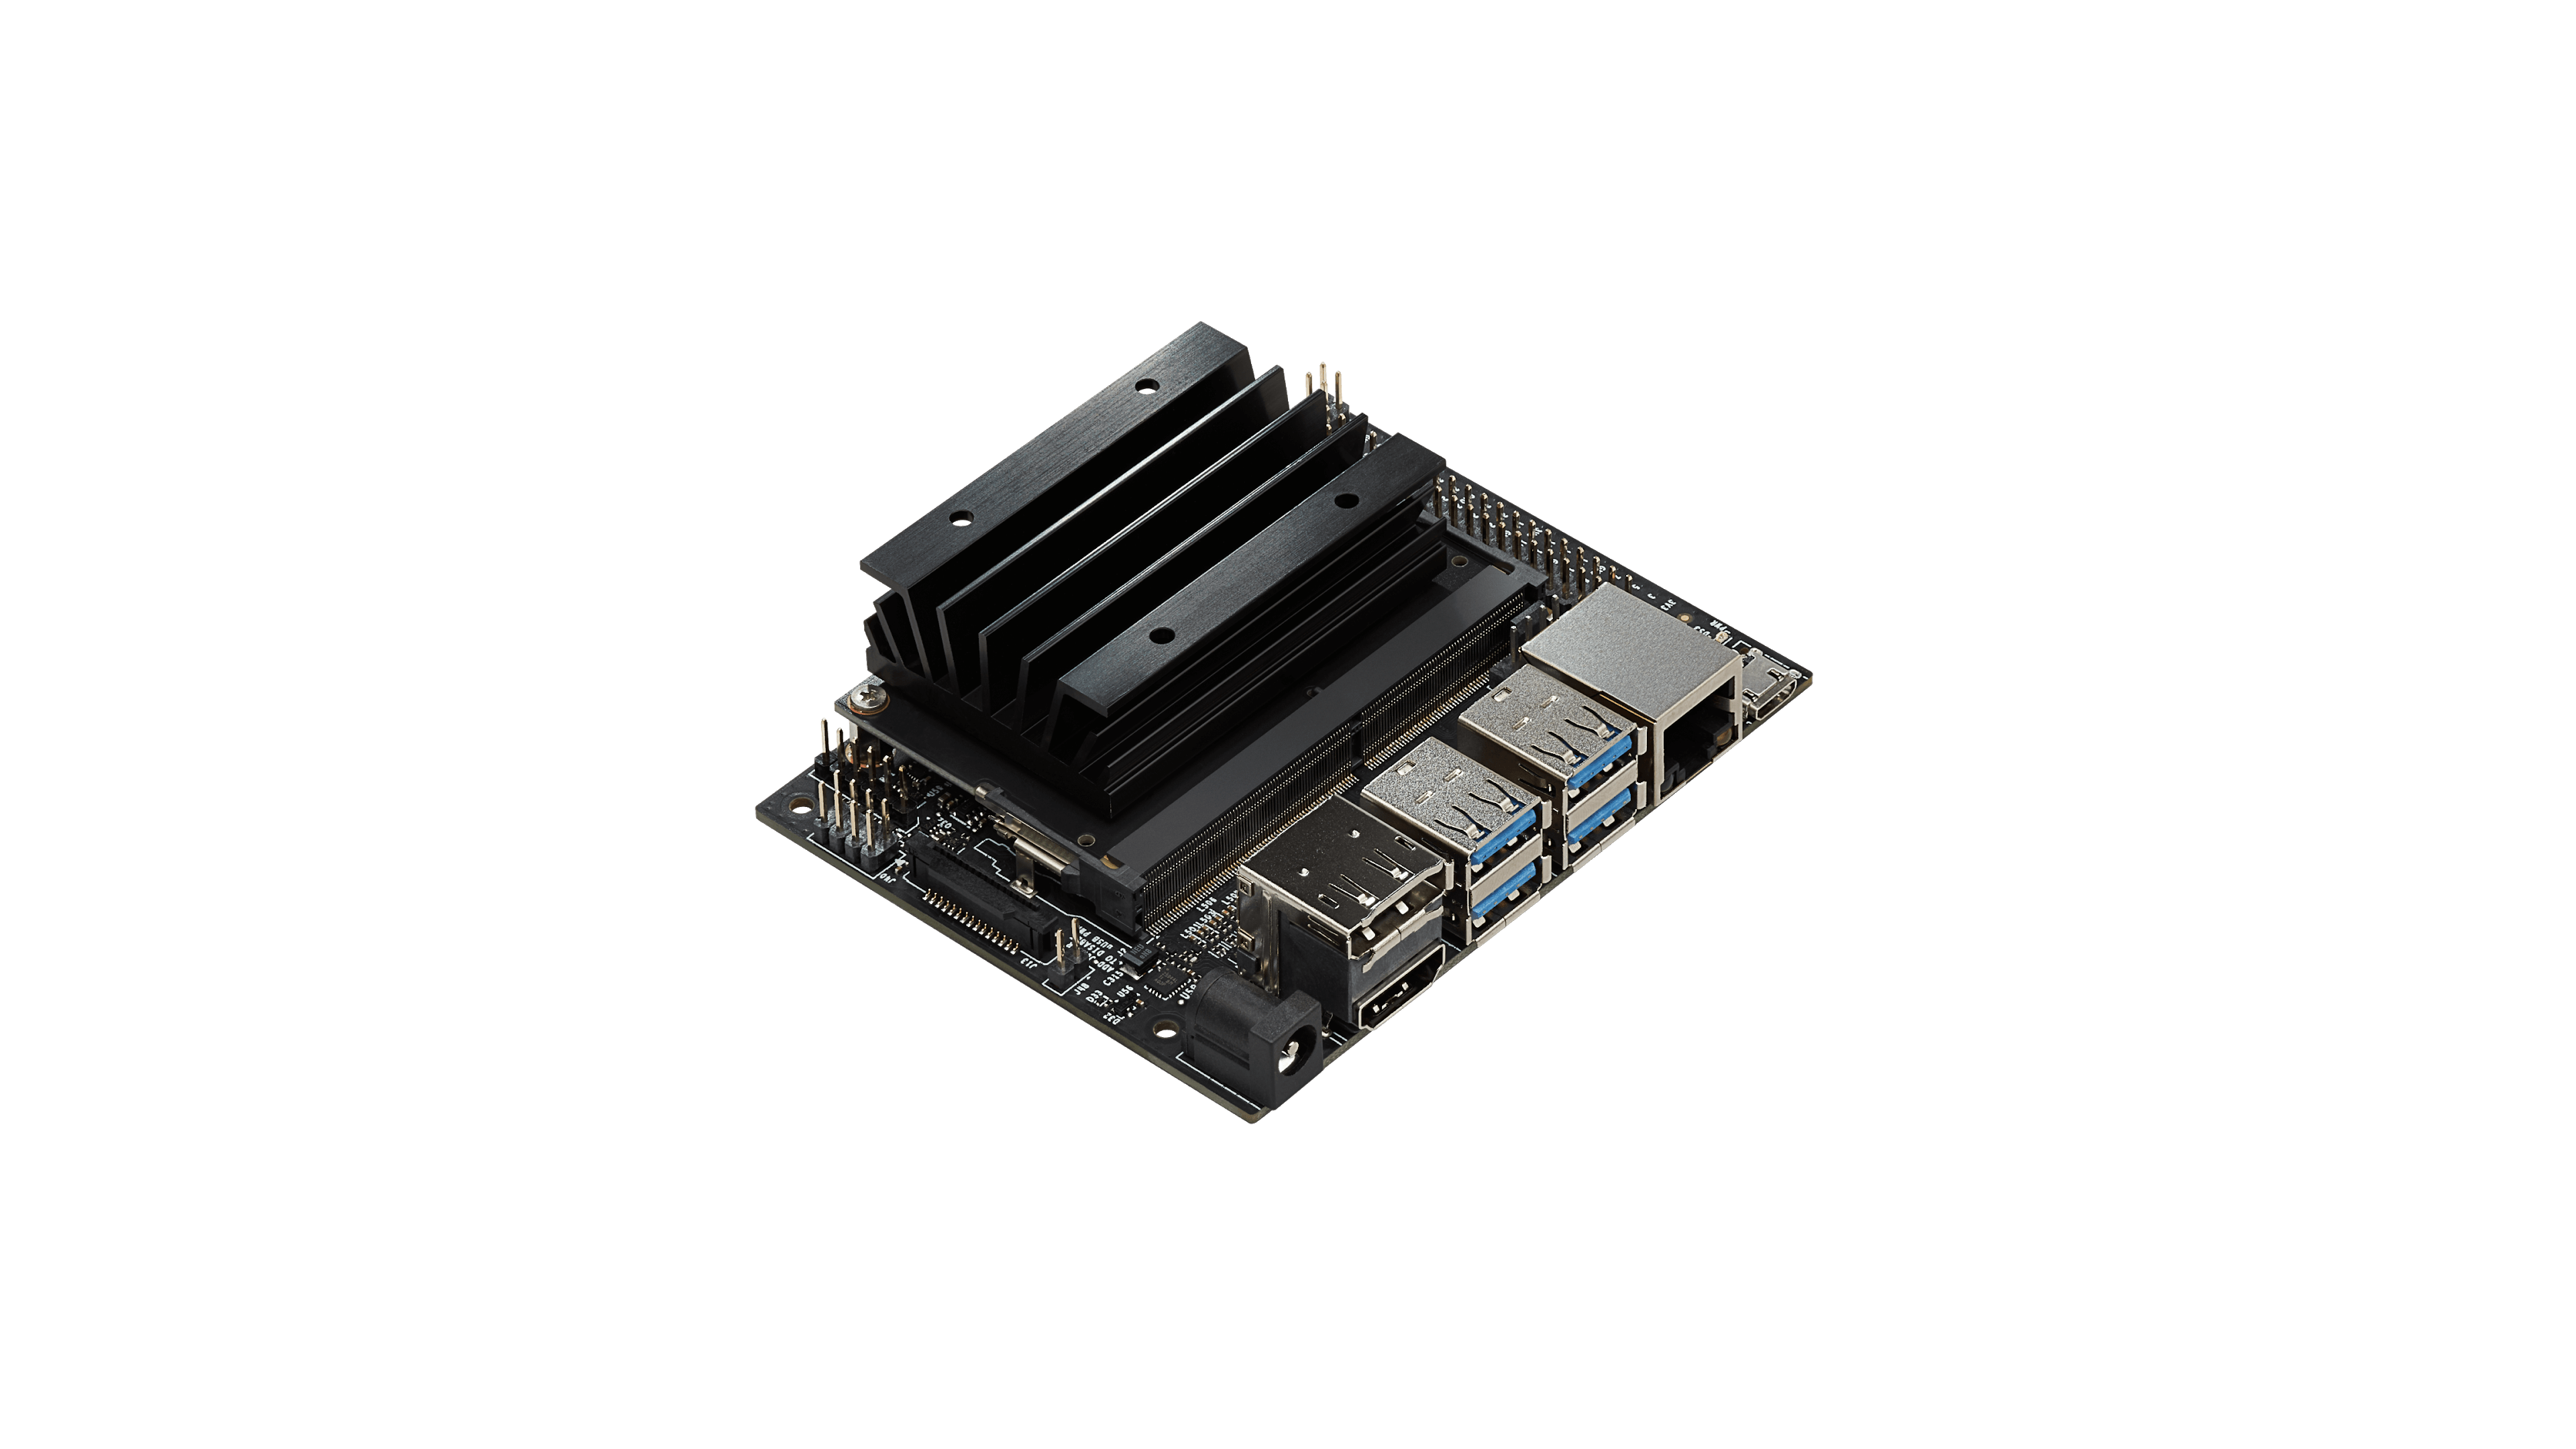
\includegraphics[width=0.4\textwidth]{img/jetson-nano.png}
        \caption{Jetson Nano}
        \label{fig:jetson}
    \end{figure}

    \noindent The project has been developed using the C++ programming language and the CUDA library. 
    The CUDA library has been used to exploit the GPU capabilities and to perform the image processing operations in parallel.

    \subsection{Program's history}
    The project has been developed gradually. The first version of the project $(v0.5)$ has been developed on January 19th. 
    This version implemented the image processing operations using three different CUDA functions, one for each operation. 
    This operating mechanism slows down the execution of the program because the image is copied back and forth three times between GPU and CPU memory,
    other than suffering from the overhead of the CUDA function calls and kernel creation.
    Moreover, there are black borders around the image, which create a worse looking image when the borders are enlarged.
    In $v0.5$ the final image has square dimensions, since the complete zooming feature has not been implemented yet.

    The second version of the project $(v0.9)$ has been developed on January 26th. It encapsulates the three image processing operations in a single CUDA function,
    which is called only once, making the execution faster and reducing the overhead of the CUDA function calls and kernel creation. 
    This version of the project still implements the black border around the image.
    Moreover, it implements a complete zooming feature, which allows the user to zoom in by selecting a rectangular area of the image.

    The third and final release of the project $(v1)$ has been developed on February 10th.
    This version removes black edges around the image using the technique explained in the previous section, producing a better looking output when the image is zoomed near the edges. 

    
    \subsection{Results comparison}
    All three versions have been analyzed and compared in terms of execution time and image quality. Moreover, the profiling of the code has been performed to understand the bottlenecks, while 
    also trying to make fully use of the calculator's capabilities. 
    These results are presented in the following table \ref{tab:expres}.
    % Tabella con i risultati   
    \small
    \begin{table}[ht]
        % \begin{tabular}{|p{1.5cm}|p{4cm}|p{2cm}|p{2.5cm}|p{2.5cm}|}
        \begin{tabular}{|c|c|c|c|}
            \hline
            Version & Global/Shared memory& Time to execute (s) & Shared ld/st conflicts \\
            \hline
            v0.5 (19 Jan) & Shared & 3.09 & 0\\
            \hline
            v0.9 (26 Jan) & Global & 0.495 & /\\
            \hline
            v0.9 (26 Jan) & Shared & 0.460 & 0\\
            \hline
            v1 (10 Feb) & Global & 0.148 & /\\
            \hline
            v1 (10 Feb) & Shared & 0.137 & 0\\
            \hline
        \end{tabular}
        \caption{Experimental results}
        \label{tab:expres}
    \end{table}
    The main notable difference in the table between the 3 version is the execution time of the program. This is due to the fact that the first version of the project uses three different CUDA functions,
    as explained in the previous section. This is also due to a poorer use of GPU capabilities. 
    The second version achieves a speedup of 6.2x with respect to the first one, while the third version achieves a speedup of 21x.
    This speedup is achieved thanks to the substitution of the if-else clauses with the use of mathematical operations for computing of indexes.
    
    The following [\ref{fig:original}] is the original image used to test the project. The image is a 640x426 pixels image, which is a typical resolution for a mid-range smartphone camera.
    \begin{figure}[h]
        \centering
        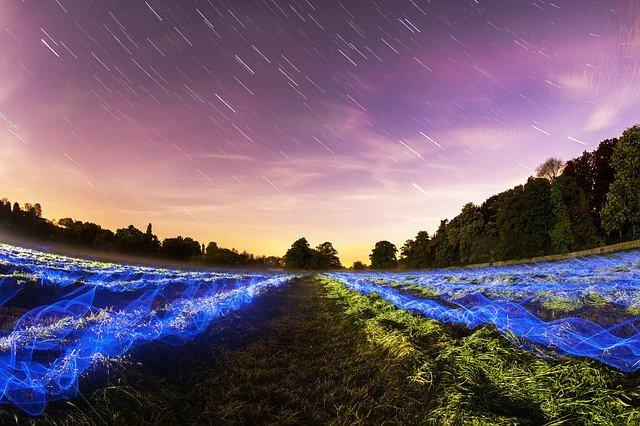
\includegraphics[width=0.5\textwidth]{img/start/sample640x426.jpg}
        \caption{Original image}
        \label{fig:original}
    \end{figure}

    \noindent The following [\ref{fig:zoom}] shows the zoomed image using the last version of the project. 
    On the left side, the original image is shown, with a zoom performed one the selected area, without the use of a filter.
    On the right side, the zoomed image is shown, with the use of a Gaussian filter of size $15x15$ and a standard deviation of 5.

    \begin{figure}[h!]
        \centering
        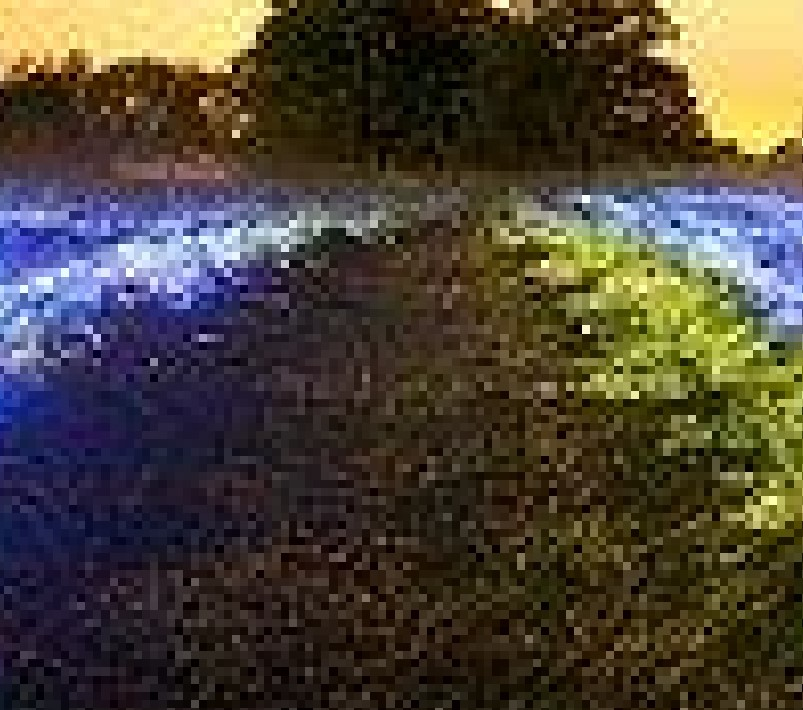
\includegraphics[width=0.455\textwidth]{img/start/selectedZoneZoom.jpg}
        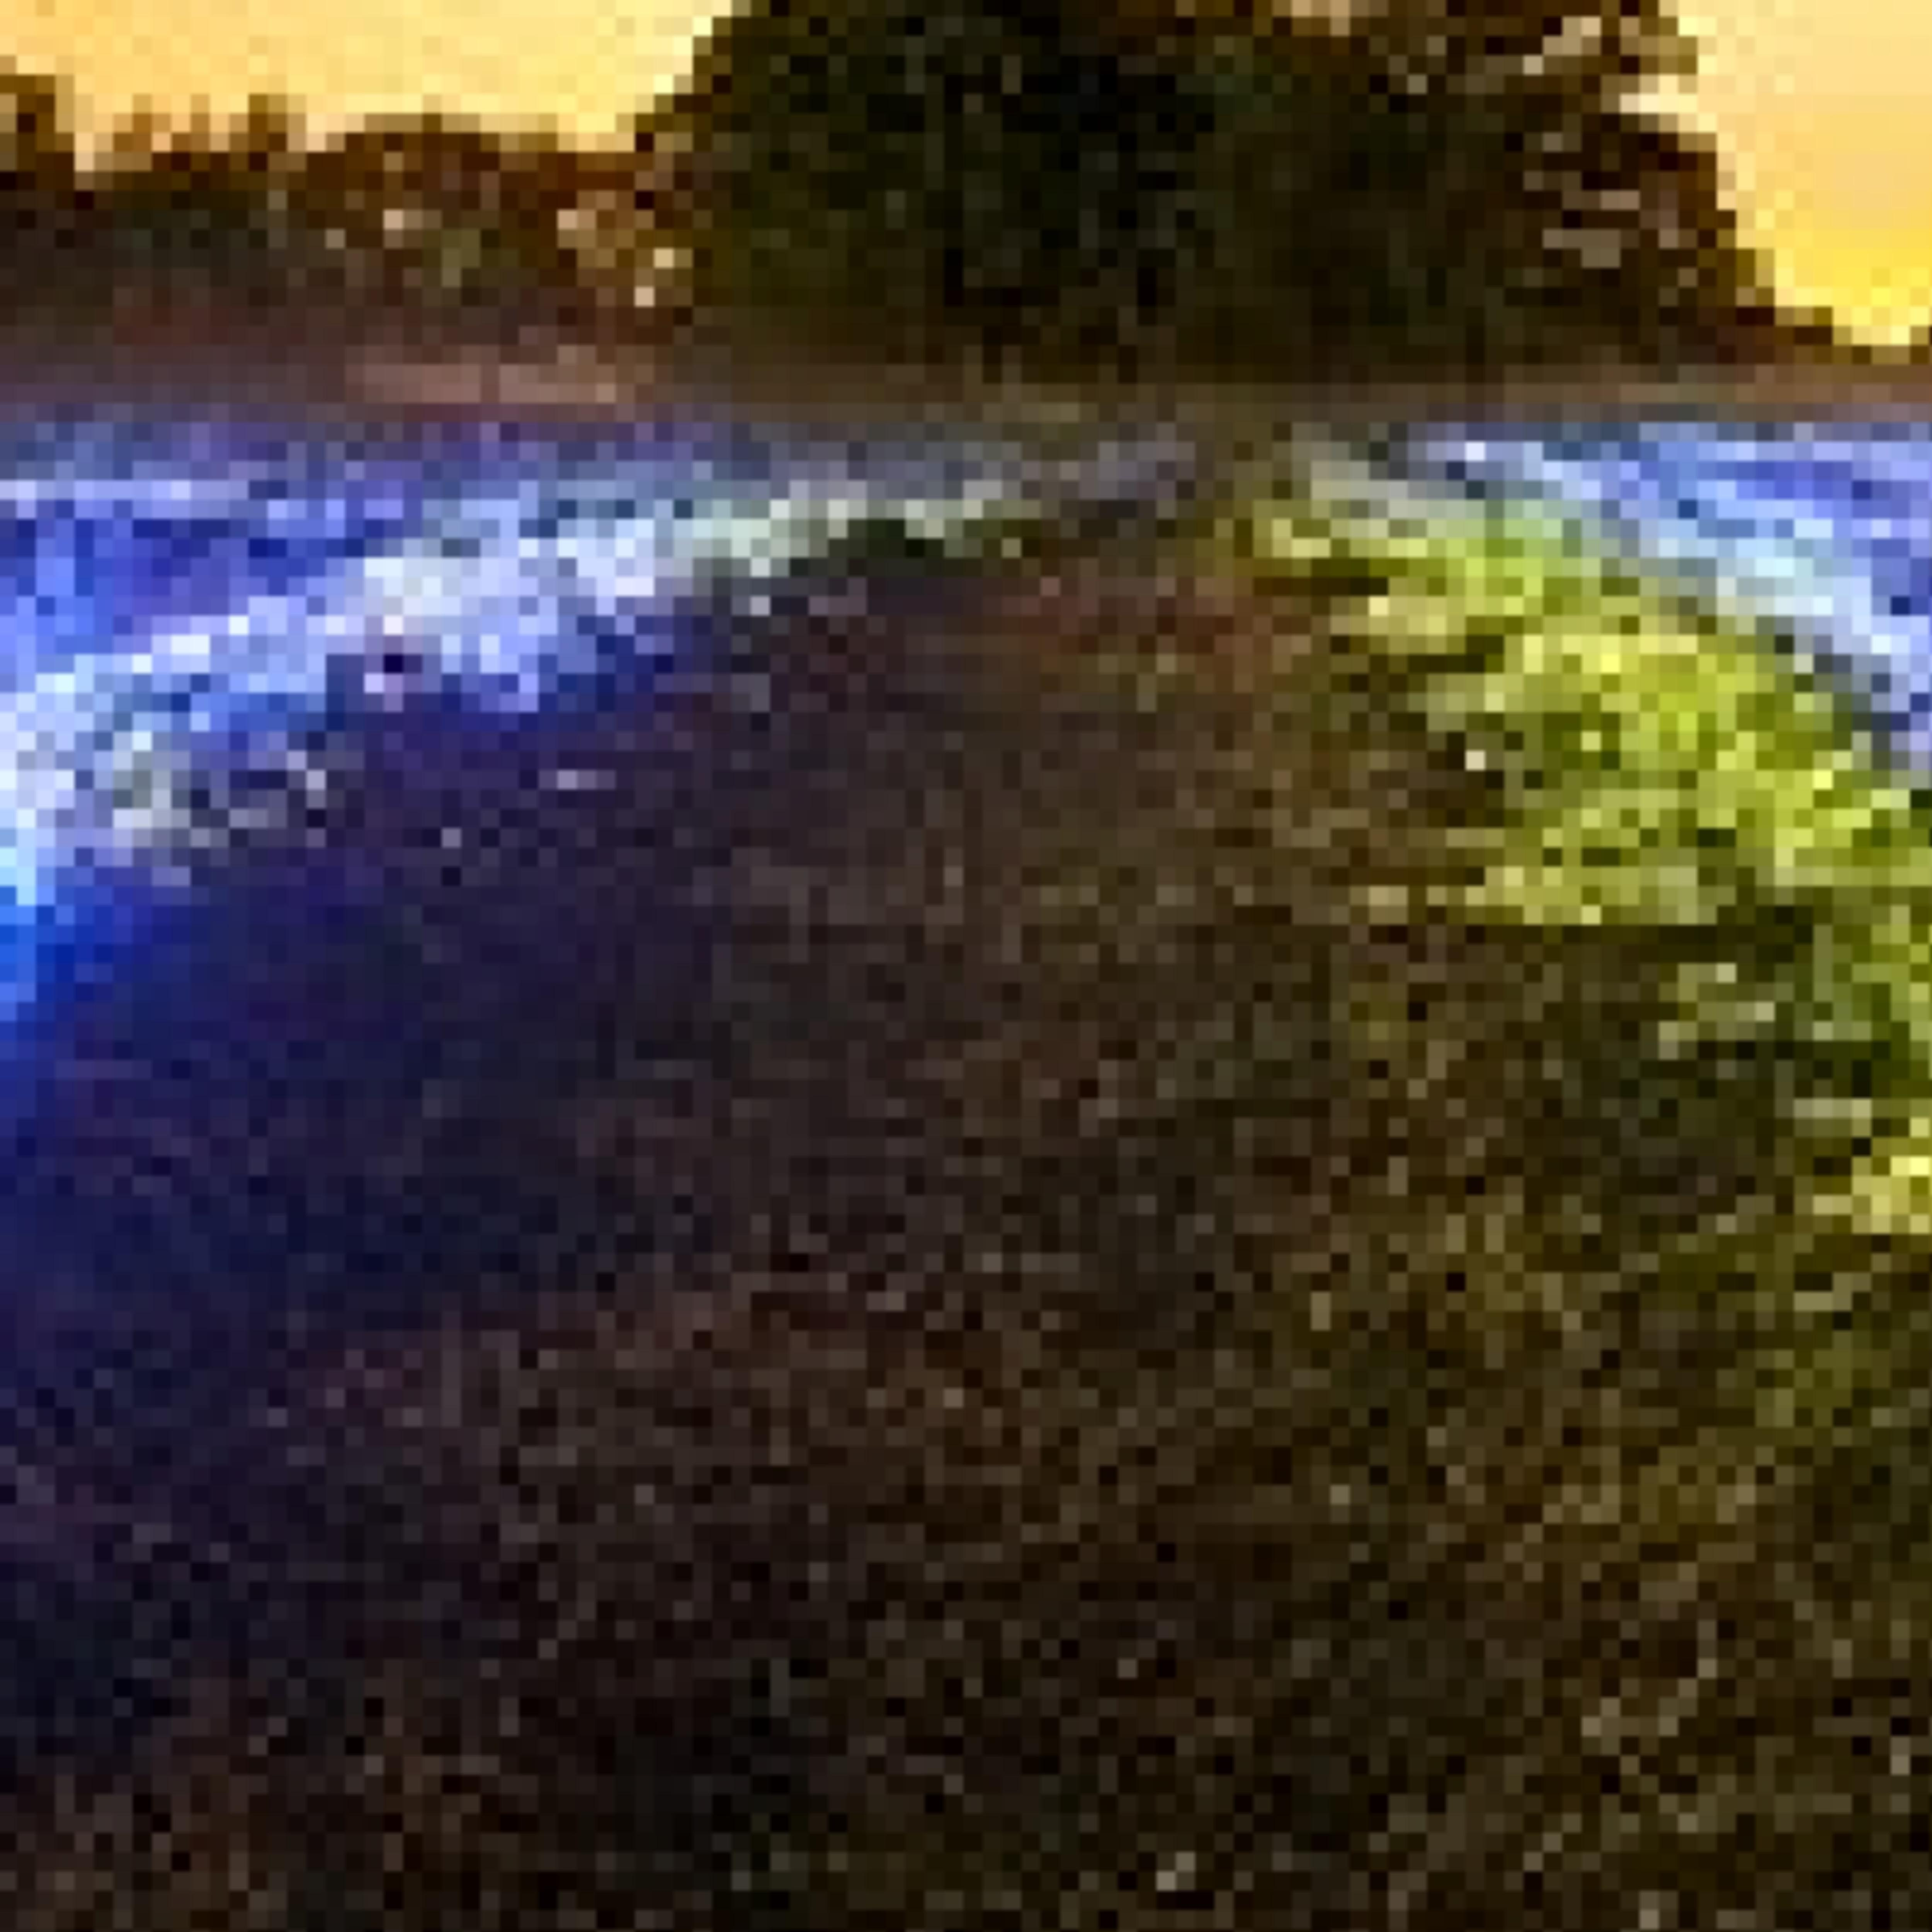
\includegraphics[width=0.4\textwidth]{img/start/selectedZoneCutout.jpg}
        \caption{Zoom in the original image \& and zoomed image using v1}
        \label{fig:zoom}
    \end{figure}

    Using the Jetson Nano to achieve maximum performances and to fully exploit the GPU capabilities, the Watchdog timer was disabled, which is a feature that 
    automatically stops hanging processes. This feature is enabled by default, and stops the execution after 5s of activity of a single thread.
    The discovered limits of the Jetson Nano have been found to be a maximum resolution of 5000x5000, using a Gaussian kernel of size $15x15$,  
    while keeping the same size of the original image ($640x420$), the maximum Gaussian kernel size which can be reached is found to be 111x111.
    Obviously these numbers are not the upper limit in every occasion, but they're the maximum possible for the image used in the test.

    \subsection{Using custom kernel masks}
    Gaussian kernel are used to blur the image, mainly to reduce the noise, obtaining a smoother picture from the convolution, ideal after
    enlarging it. Other types of more suitable masks can be used for other purposes.
    The examples shown down below are the results of kernels convoluted to execute embossing \cite{custom_kernels_a}, 
    edge detection, ridge detection \cite{custom_kernels_b} and darkening/lightening of the image.

    In figure \ref{fig:emboss} the embossed image is shown. The embossing is a technique used to create a 3D effect on a 2D image, 
    by using a specific kernel. The 3D effect of the image shows the depth of the pixel. Every colour has a different depth, going from black, the deepest, 
    to white, the narrowest.
    \begin{figure}[h]
        \centering
        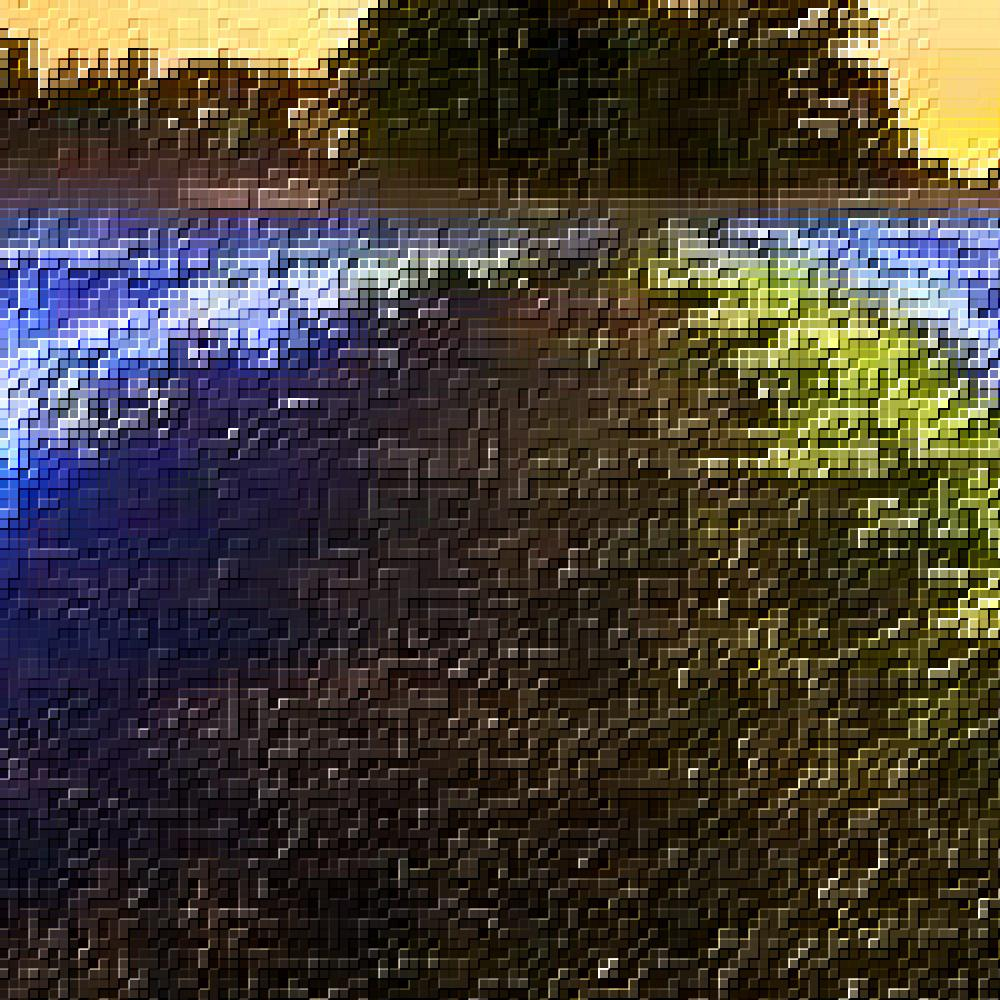
\includegraphics[width=0.4\textwidth]{img/emboss/final.jpg}
        \caption{Embossed image}
        \label{fig:emboss}
    \end{figure}


    In figure \ref{fig:darken_lighten} the darkened and lightened images are shown. 
    The darkened image is obtained by using a $3x3$ kernel which contains as center a value between $0$ and $1$, 
    because it reduces the value of all the pixels in the image. The lightened image is obtained by using a $3x3$ kernel which contains as center a value greater than $1$,
    because it increases the value of all the pixels in the image, given the multiplication used by the convolution.
    \begin{figure}[h]
        \centering
        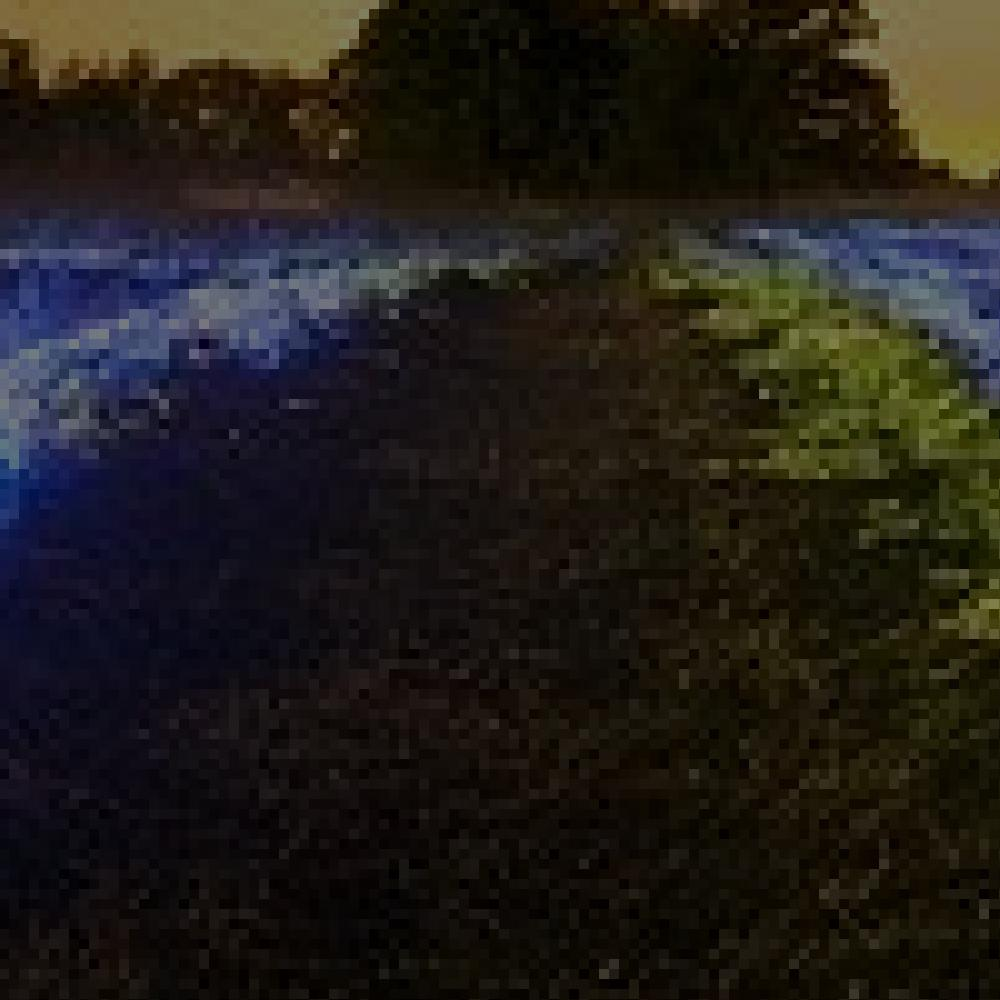
\includegraphics[width=0.4\textwidth]{img/darken_lighten/final_darken.jpg}
        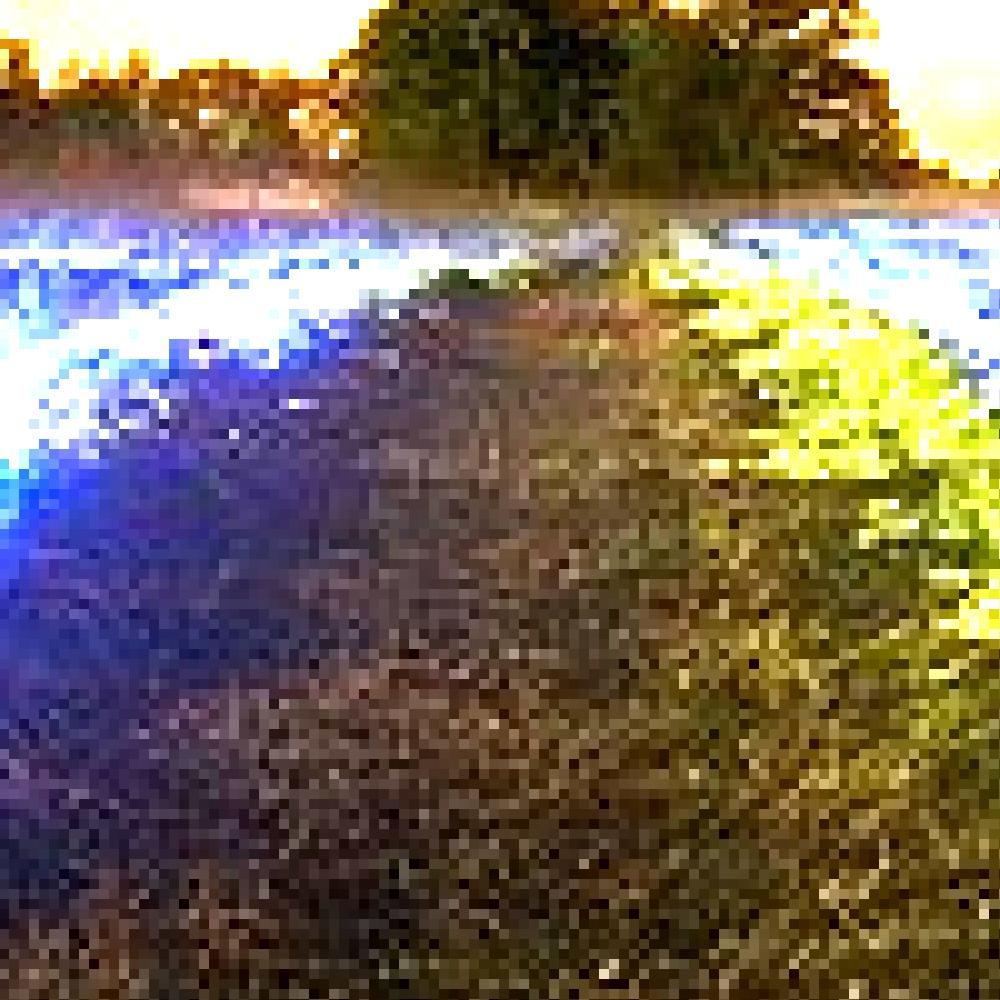
\includegraphics[width=0.4\textwidth]{img/darken_lighten/final_lighten.jpg}
        \caption{Darkened image \& Lightened image}
        \label{fig:darken_lighten}
    \end{figure}

    The last two alternative kernels used in this project are for edge and ridge detection.
    They do the same thing, but the difference is that edge detection is more sensitive to changes, meaning that a sudden change in the colour of the pixel, 
    remaining in the same color space, is detected as an edge. Ridge detection is less sensitive, it is more focused on changes between different colours, achieving 
    a better result in detecting the edges of objects, or, in the case of the image used in the test, the edges between the sky and the trees, as well as those 
    between the lights in the grass and the grass itself. The previous, instead, detects edges between each curve in the grass and the light.
    \begin{figure}[h]
        \centering
        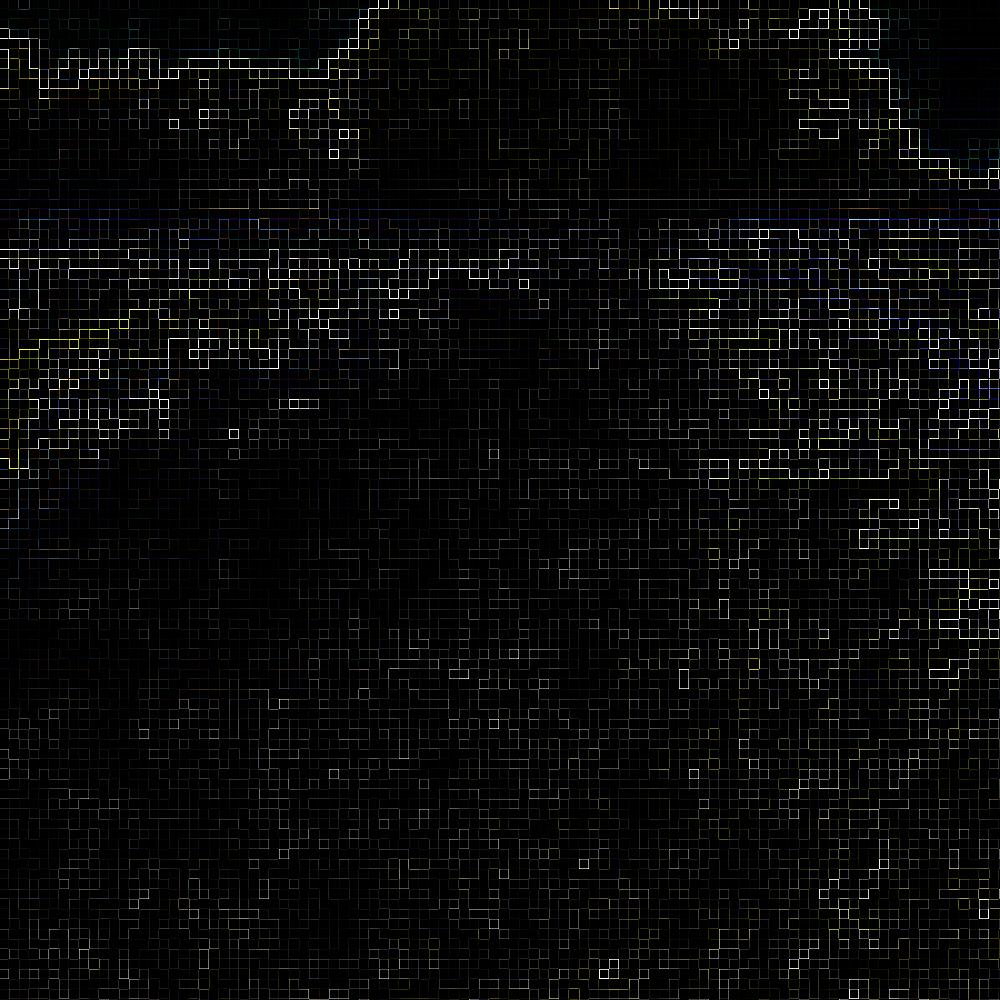
\includegraphics[width=0.4\textwidth]{img/edgedet/final.jpg}
        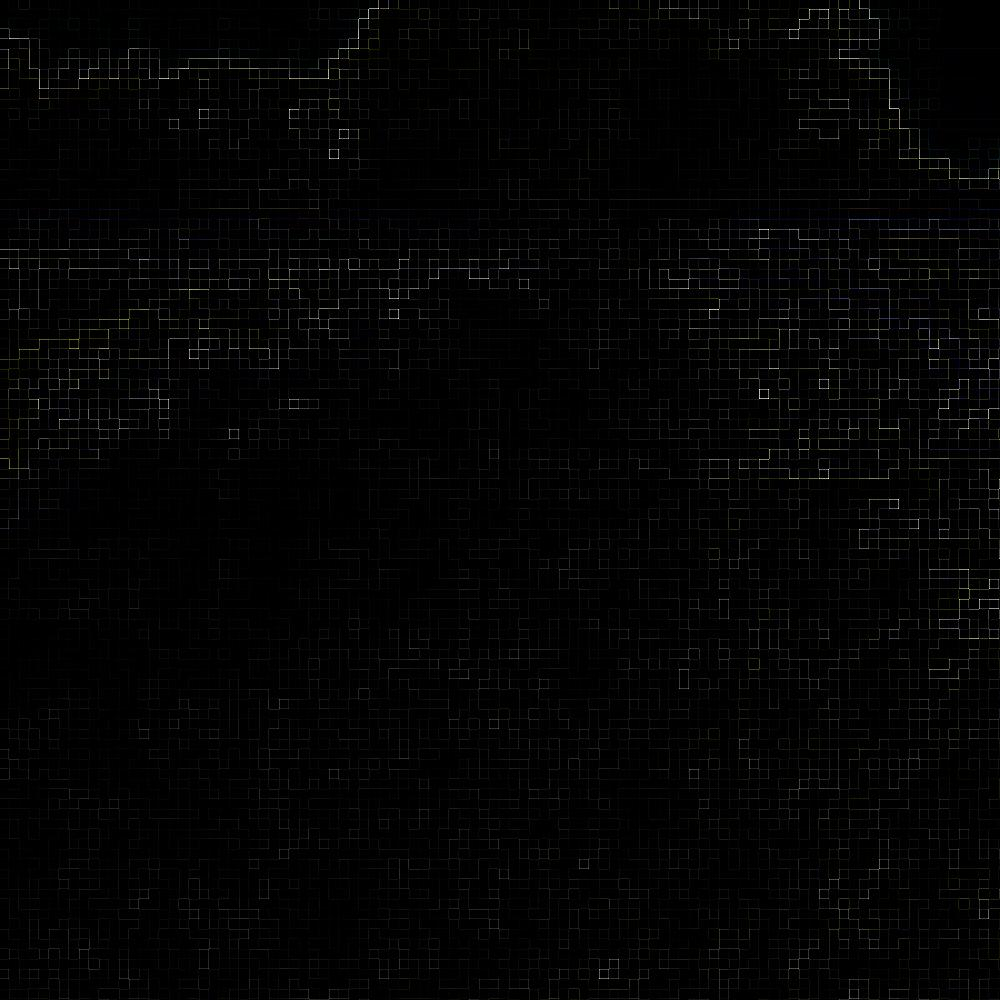
\includegraphics[width=0.4\textwidth]{img/ridge/final.jpg}
        \caption{Edge detection \& Ridge detection}
        \label{fig:edge}
    \end{figure}

\clearpage